% !TeX spellcheck = en_US
\documentclass{article}
\usepackage[english]{babel}
\usepackage[utf8]{inputenc}
\usepackage{fancyhdr}
 \usepackage{xcolor}
 \usepackage{lmodern}
 \usepackage{listings}
 
\usepackage{graphicx}
 \lstset{language=[90]Fortran,
 	basicstyle=\ttfamily,
 	keywordstyle=\color{blue},
 	commentstyle=\color{green},
 	morecomment=[l]{!\ }% Comment only with space after !
 }

\usepackage{color}
\definecolor{deepblue}{rgb}{0,0,0.5}
\definecolor{deepred}{rgb}{0.6,0,0}
\definecolor{deepgreen}{rgb}{0,0.5,0}

% Default fixed font does not support bold face
\DeclareFixedFont{\ttb}{T1}{txtt}{bx}{n}{10} % for bold
\DeclareFixedFont{\ttm}{T1}{txtt}{m}{n}{10}  % for normal

% Python style for highlighting
\lstset{
		language=Python,
		basicstyle=\ttm,
		otherkeywords={self},             % Add keywords here
		keywordstyle=\ttb\color{deepblue},
		emph={__init__},          % Custom highlighting
		emphstyle=\ttb\color{deepred},    % Custom highlighting style
		stringstyle=\color{deepgreen},
		frame=tb,                         % Any extra options here
		showstringspaces=false            % 
}





\pagestyle{fancy}
\fancyhf{}
\lhead{Vincenzo Maria Schimmenti - 1204565}
\rhead{\today}
\rfoot{Page \thepage}
\lfoot{Exercise 4}
\title{%
	Information Theory and Computation \\
	Exercise  4}
\author{Vincenzo Maria Schimmenti - 1204565}
\begin{document}
\maketitle
 
\section*{Code Development and Results}
\subsection*{Multi-run scripts}
The first part of the exercise asked to exploit a fortran code for matrix multiplication, a python script and gnuplot to plot the execution time of different methods for matrix multiplication. In order to pass to the fortran code the matrix size we wanted to probe we used:
\begin{lstlisting}[language=Fortran]
if(COMMAND_ARGUMENT_COUNT() < 1)then
	nn = 100
else
	call GET_COMMAND_ARGUMENT(1, nnchar)
	read(nnchar,FMT=*, IOSTAT=stat)nn
	if((stat.NE.0).OR.(nn <= 0))then
		nn = 100
	end if	
endif
\end{lstlisting}
This code checks if an input is given for the matrix size; if not it sets the size to the default one which is 100. The fortran code then prints line by line the execution times of all 7 methods used for multiplication (the six naive loop ones and the intrinsic one).The python script takes 3 input command line arguments, $N_{min}$ and $N_{max}$ which are the lowest and highest matrix sizes to probe and $N_{count}$ which counts the number of sizes; this is done via:
\begin{lstlisting}[language=Python]
if(len(sys.argv) >= 4):
	N_min = int(sys.argv[1])
	N_max = int(sys.argv[2])
	N_count = int(sys.argv[3])
else:
	N_min=50
	N_max=1500
	N_count = 50
\end{lstlisting}
The sizes are computed using a log scale:
\begin{lstlisting}[language=Python]
sizes = np.logspace(np.log10(N_min),np.log10(N_max+1),num=N_count,dtype=int)
\end{lstlisting}
and the execution time are stored in the following way:
\begin{lstlisting}
times = np.zeros((len(sizes),7))
fName = 'matrixmul.x'
modes = ['ijk','ikj','jik','jki','kij','kji']
for i,sz in enumerate(sizes):
	print('%.2f' % float(i*100/len(sizes)),'%')
	print('Matrix size:',sz)
	result = subprocess.run(['./'+fName,str(sz)], stdout=subprocess.PIPE)
	splits = result.stdout.decode('utf-8').lstrip().split('\n')
	times[i,:]=np.array([float(tm) for tm in splits[0:7]])
\end{lstlisting}
We use the \textit{subprocess} module to launch the fortran program with proper command line arguments; the output is read and then stored into different files. These files are then read by a gnuplot script which employs the \textit{for loop} of the \textit{plot} command.; the file names are hard coded into the script itself. The resulting (log) plot is:
\begin{center}
	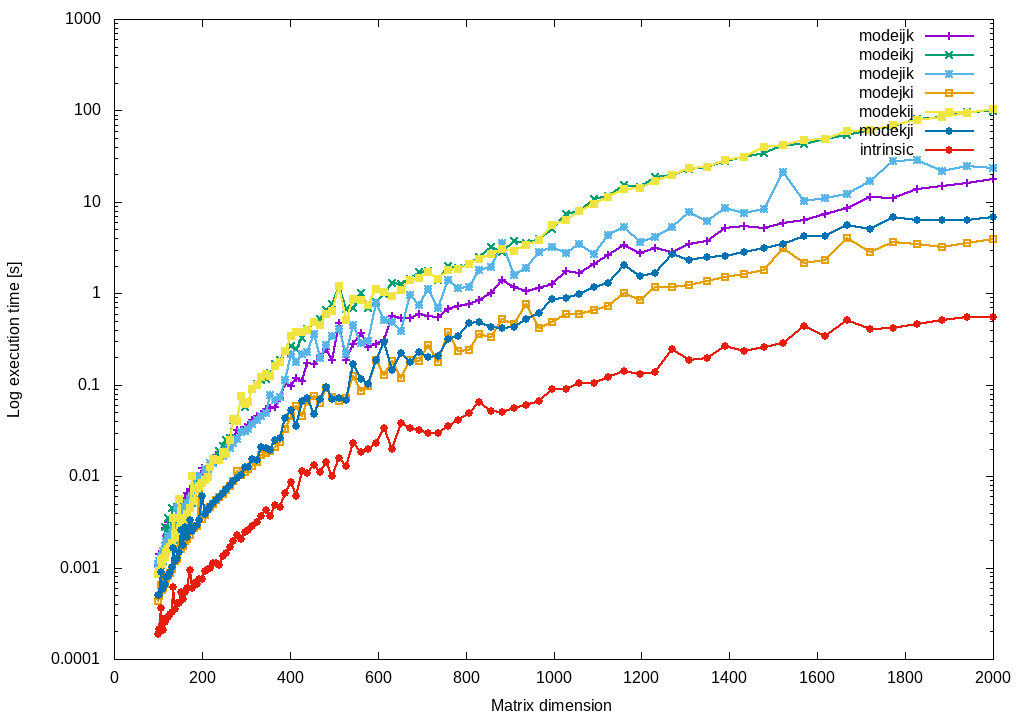
\includegraphics[width=0.65\linewidth]{time_plots.png}
\end{center}
As expected the intrinsic method is way better scalable; we clearly see in the other plots how exploiting the cache can help speed up the algorithm.
\subsection*{Automated fits}
The second part of the exercise consisted in fitting the curve of the previous part using gnuplot and automatizing this fitting procedure using python. In order to do so a gnuplot script has been written (\textit{timefit.plt}) which reads from a file (\textit{file\_to\_fit.txt}) the name of the file containing the data to fit and outputs the parameters of the fit; the script must be run as \textit{gnuplot timefit.plt}. We made this procedure automatic by hard coding the file names into a python script and by writing theese names one by one into the aforementioned file; then, by using the \textit{subprocess} module, the script launches the gnuplot one. As a demonstration we show below an one of the obtained fits:
\begin{center}
	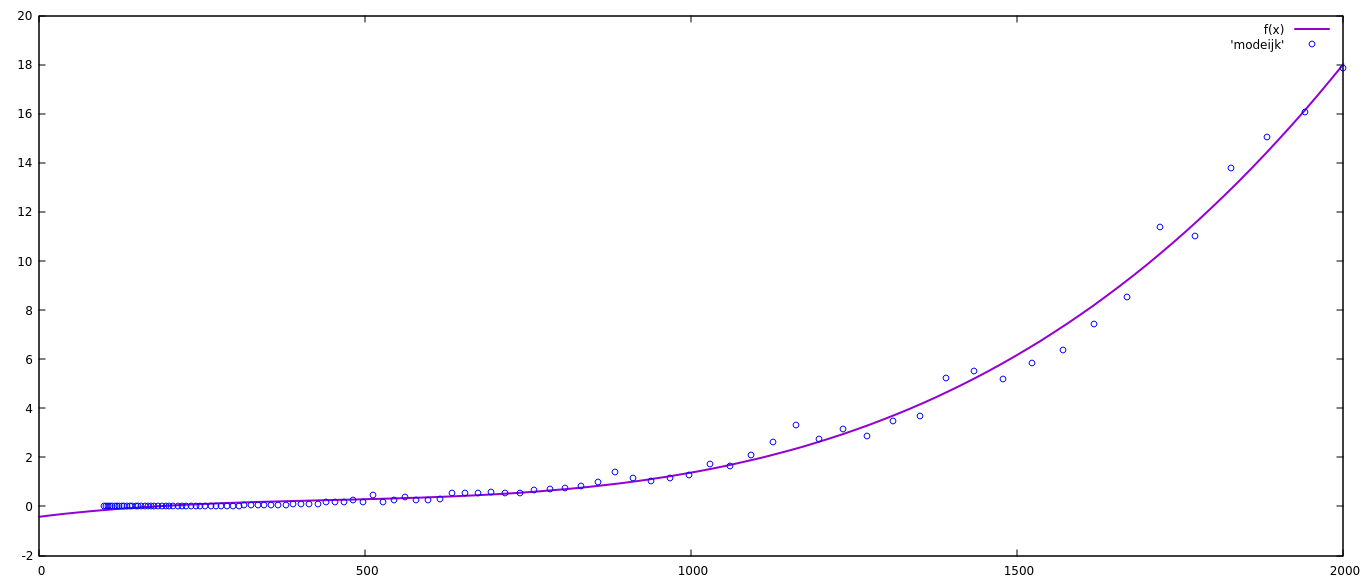
\includegraphics[width=0.8\linewidth]{examplefit.png}
\end{center}
\end{document}